\section{Web UI Investigation Tool}\label{section-investigation-tool}

The web application is designed as a single page web-application, such that changes in the URL represent the application rendering a different view dynamically, rather than making a request for a new web-page. 

\subsection{Technology Choices}
\subsubsection{Angular 6 \& TypeScript}
Angular 6 provides excellent tooling for scaffolding out a wire-frame for the application and scaffolding out individual components. This is achievable using the \texttt{@angular-cli} tool where a command as simple as \texttt{ng new my-app; cd my-app; ng serve} will have a wire-frame web application up and running. This was a lucrative feature of Angular for this project, since it would help expedite the web-application setup process and facilitate more time to be spent on developing features.
\\\\
Angular 6 applications are written in TypeScript; a statically typed super-set of JavaScript. Using a statically-typed language is a personal preference of mine, where possible, in order to allow for some compile time type-checking and easier refactoring. 
\\\\
Angular comes with RxJS, an asynchronous programming library. This provides a new approach to asynchronous requests than simple Promises in JavaScript, which can only be subscribed to once. RxJS provide Observables which can be subscribed and listened to indefinitely and provide any number of date updates. This is particularly useful for my application since every interaction the user makes with the graph will initiate an asynchronous request to fetch the data to render further nodes/information. These requests may be made concurrently too, so having a single Observable to listen for all new 'block' or 'transaction' information, for instance, would greatly simplify my implementation. 
\\\\
\textbf{Alternatives to Angular}: React is another solution to building single-page web-applications that is popular in the industry. However, React is a library whereas Angular is a fully-fledged MVC framework providing far more 'out-the-box' functionality. React only provides the 'V' (the view) and will require several other libraries to fill in the model and controller components of MVC. Due to my familiarity with Angular, and comparatively unfamiliar with React, there would potentially be a steep learning curve adopting React for this project, in addition to the several libraries I may require to integrate with. Angular would allow me to build and iterate fast since much of the basic functionality is provided by Angular.

\subsubsection{D3}
D3.js is a JavaScript library that can be used for generating SVG visualisations in the DOM. D3 has no direct connection to Neo4J, unlike some other tools. The data will therefore be retrieved using my own database API and will therefore involve further steps to fetch the data to render; however, this is advantageous as it will provide the flexibility to customise the API implementation to orchestrate responses by making customised queries or communicating with several data stores.
\\\\
\textbf{Alternatives to D3}: There exist some visualisation tools that have embedded connections to Neo4J. I initially considered these tools as a possible simplification of the visualisation element of the web application; however, these tools such as Neovis.js and Popoto.js seem too restrictive in that their data format must align with the data format in Neo4J. They appear to be very suitable for visually mirroring the data in Neo4J, but I believe for this project, with the scope for many visual features with data persisted in locations other than Neo4J, this will prove to be too constraining. As for other JavaScript libraries similar to D3 with high customisability, I chose D3 due to the abundance of documentation, community support and example projects that D3 has. 

\subsection{Implementation}
The most significant features provided by Angular that I used throughout the project were:
\begin{itemize}
    \item \textbf{Components \& Templates} - specifically: two-way data binding. The template will render the data defined in the component; changes to this data will lead to the template dynamically re-rendering to display the updated value. The component can listen to event hooks on the template, such as a click of a button or a value inserted, to retrieve user input/interactions from the template.
    \item \textbf{Services} - a way of communicating data within the app and externally from the app. Bitcoin service is responsible for making requests to the backend API to search for data in the database. The investigation service is largely used to communicate data across the components. For instance, the search component supplies the investigation service with search result data. This is published to an observable, which is being listened to by the investigation component which renders the new data as it arrives. Services help with separation of dependencies between components that should not need to know about each-other. 
    \item \textbf{Dependency Injection} - Injectable components (such as services) are requested by components that require them, rather than creating the dependencies them-self. This improves efficiency and modularity. 
\end{itemize}

\subsubsection{Routes}
There existed two main routes within the application:
\begin{itemize}
    \item \texttt{/search} : Loads the search component
    \item\texttt{/investigation} : Loads the investigation component (only if navigated there from the search form, otherwise it re-directs back to \texttt{/search}).
\end{itemize}

\subsubsection{Architecture}
The overall architecture of the web application can be seen in figure \ref{fig:webapp-architecture}. The components shown in the figure have the following roles:
\begin{itemize}
    \item Search Component: Renders the search forms. Validates users input, performs requests to fulfill searches using Bitcoin Service. Provides search results to Investigation Service. 
    \item Investigation Component: Subscribes to the many data streams of the Investigation Service and coordinates adding new nodes and links to the graph. 
    \item Graph Component: Listens to updates of the node/link data and updates the graph when data changes and initialises/re-starts the simulation when required. 
    \item Link Component: Exists simply as a template for the Link SVG on the Graph. Some logic around showing Output values in various currencies and timestamps. 
    \item Node Component: Handles user interactions with the nodes on the graph. Identifies hover actions and double clicks and communicates accordingly with the services to inform other components of the actions. E.g: On hover, passes the node information to the App Service for displaying in the node data component. Additionally handles the pulsing animation while a node is requesting data to render its neighbours. 
    \item Add Node Component: Provides a form for adding custom nodes to the graph. Validates form data and publishes new data to the Investigation service.  
    \item Add Link Component: Provides a form for crating a link between custom nodes in the graph and any other node. Validates the form and publishes new data to the Investigation Service. 
    \item Node Data Component: Responsible for rendering a overlay component displaying information about the node currently being hovered over. This data is published to an Observable in the App service and is subscribed to in order to receive updates. 
    \item Draggable Directive: Applies D3's draggable behaviour to a node. 
    \item Zoomable Directive: Applies D3's zoomable behaviour to the graph. 
    \item Investigation Service: Mainly supplies data to the investigation component using Observables. For example, an observable to publish address data looks like this:
    \begin{lstlisting}[breaklines=true, basicstyle=\small]
        private addressData = new BehaviourSubject(null);
        currentAddressData = this.addressData.asObservable();
        
        supplyNewAddressData(newAddressData: Address) {
            this.addressData.next(newAddressData);
        }
    \end{lstlisting}
    Then in the investigation component, a subscription to the observable will look like this:
    \begin{lstlisting}[breaklines=true, basicstyle=\small]
        this.investigationService.currentAddressData.subscribe((newAddressData: Address) => {
            //handle data update
        });
    \end{lstlisting}
    \item Bitcoin Service: Uses Angular's HTTP library to make HTTP requests to the backend API to fetch new data. The calls return an observable with generic type corresponding to the data model it will populate. For example, a call to fetch an address node is:
    \begin{lstlisting}[breaklines=true, basicstyle=\small]
        return this.http.get<Address>(this.serviceDomain + "/bitcoin/getAddress/" + address + this.buildQueryParams()); 
    \end{lstlisting}
    \item App Service: Uses observables to facilitate the transfer of data between node components and node data components. 
    \item D3 Service: Handles calls to D3 to implement Draggable and Zoomable behaviours. 
\end{itemize}

\begin{sidewaysfigure}[h!]
  \centering
  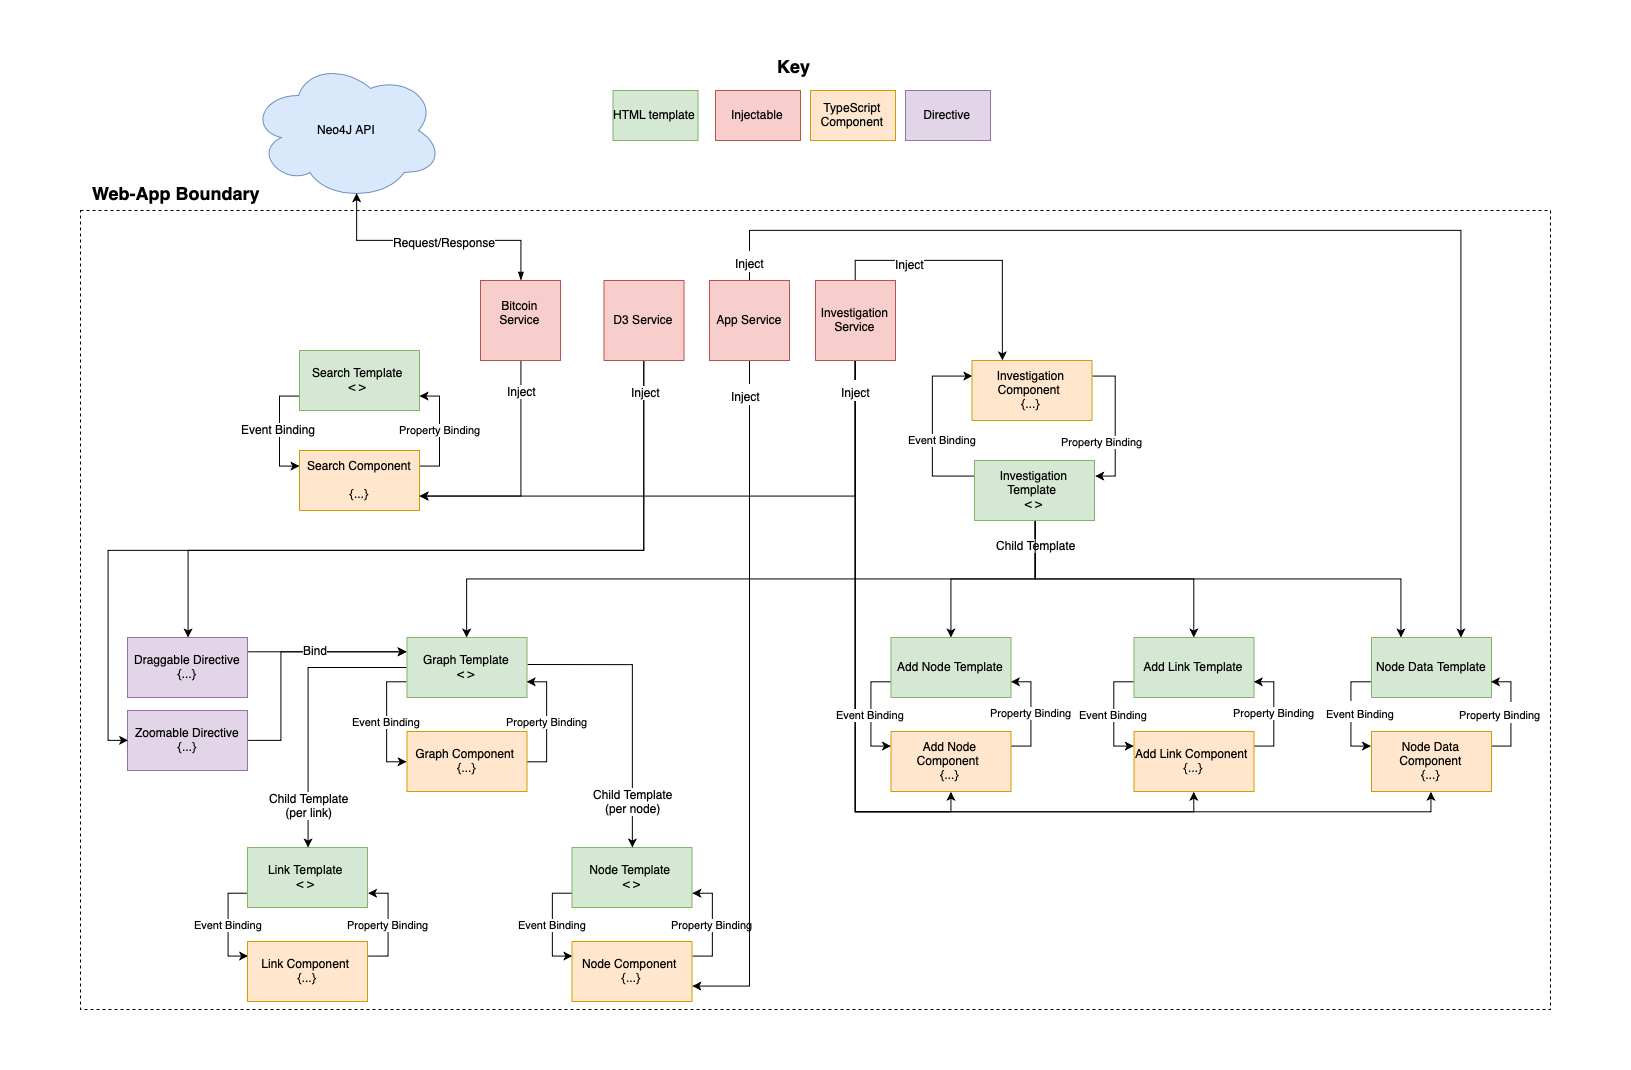
\includegraphics[width = 22cm]{./figures/webapp-architecture}\\[0.5cm]
  \caption{Architecture of the Web Application}
  \label{fig:webapp-architecture}
\end{sidewaysfigure}

\subsection{Features}
\subsubsection{Search By Address}
An investigation can be initiated by searching for a particular bitcoin address. The search form as shown in figure \ref{fig:neo4j-screenshot-search-form}, when submitted, loads the investigation view displaying the address and it's immediate neighbours as nodes in the graph, also detailing the relationship types each link represents, as shown in figure \ref{fig:neo4j-screenshot-basic-address-nodes}. 

\begin{figure}[h!]
  \centering
  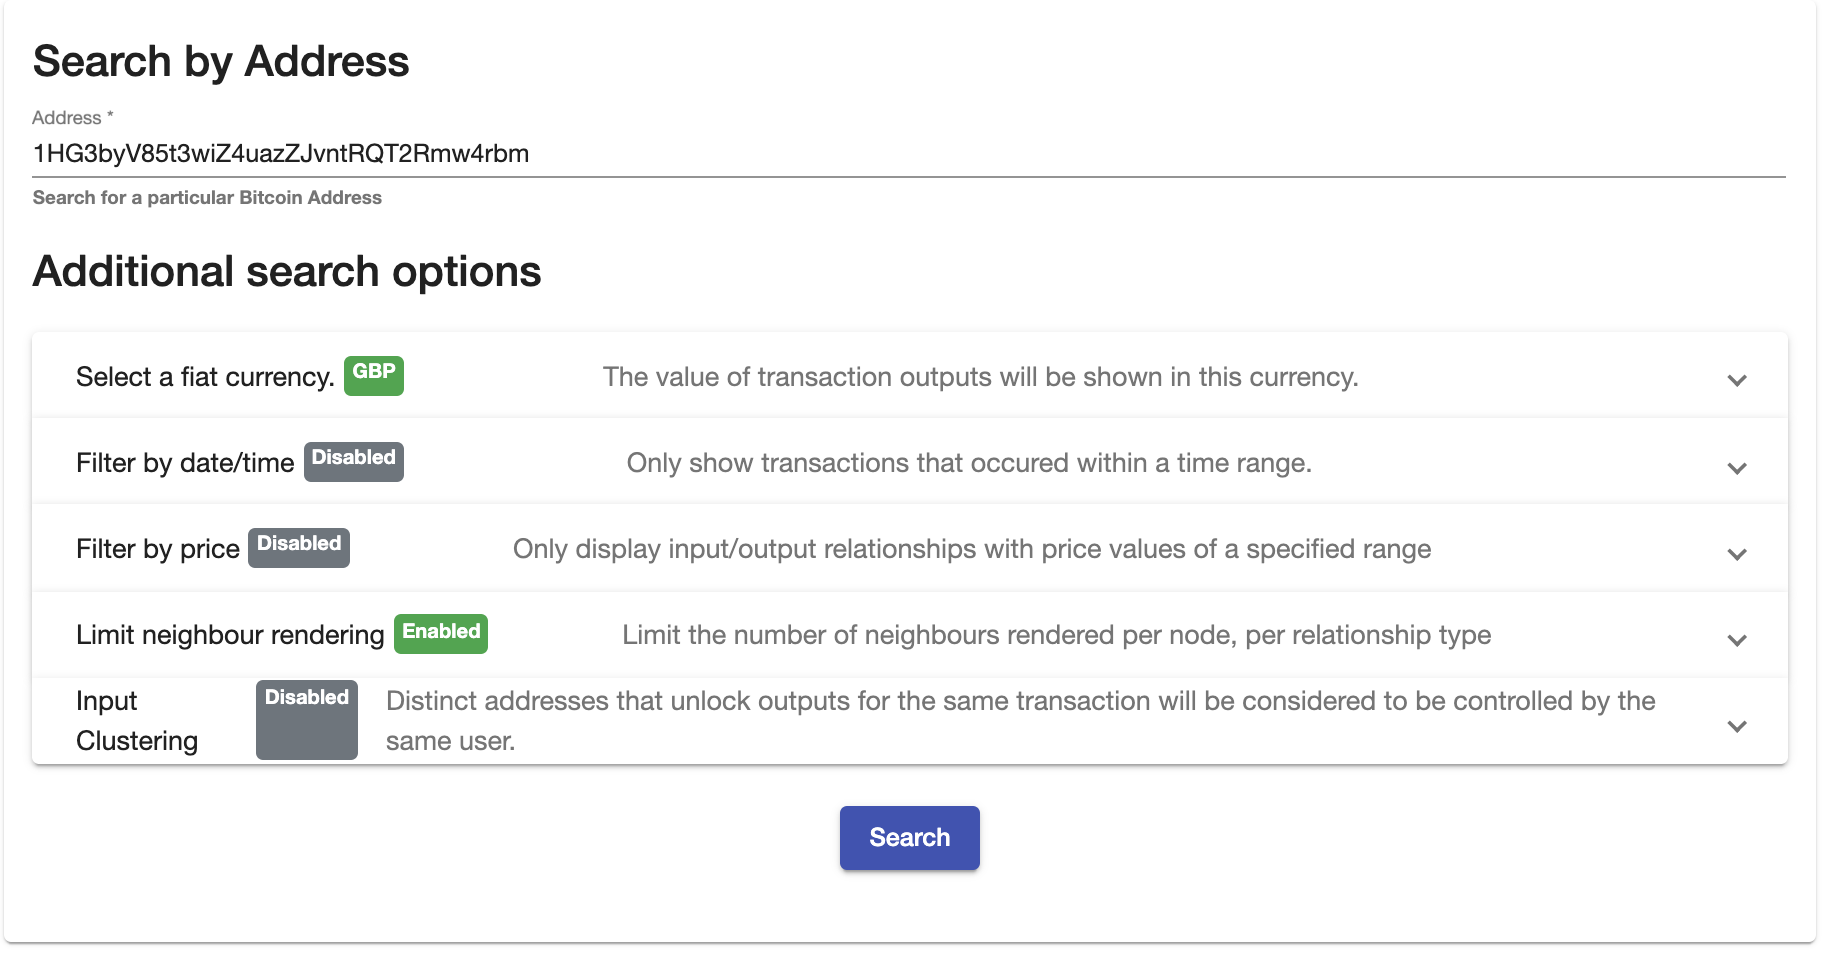
\includegraphics[width = 15cm]{./figures/ui-screenshots/search-address-form}\\[0.5cm]
  \caption{A screenshot of the address search form feature.}
  \label{fig:neo4j-screenshot-search-form}
\end{figure}

\begin{figure}[h!]
  \centering
  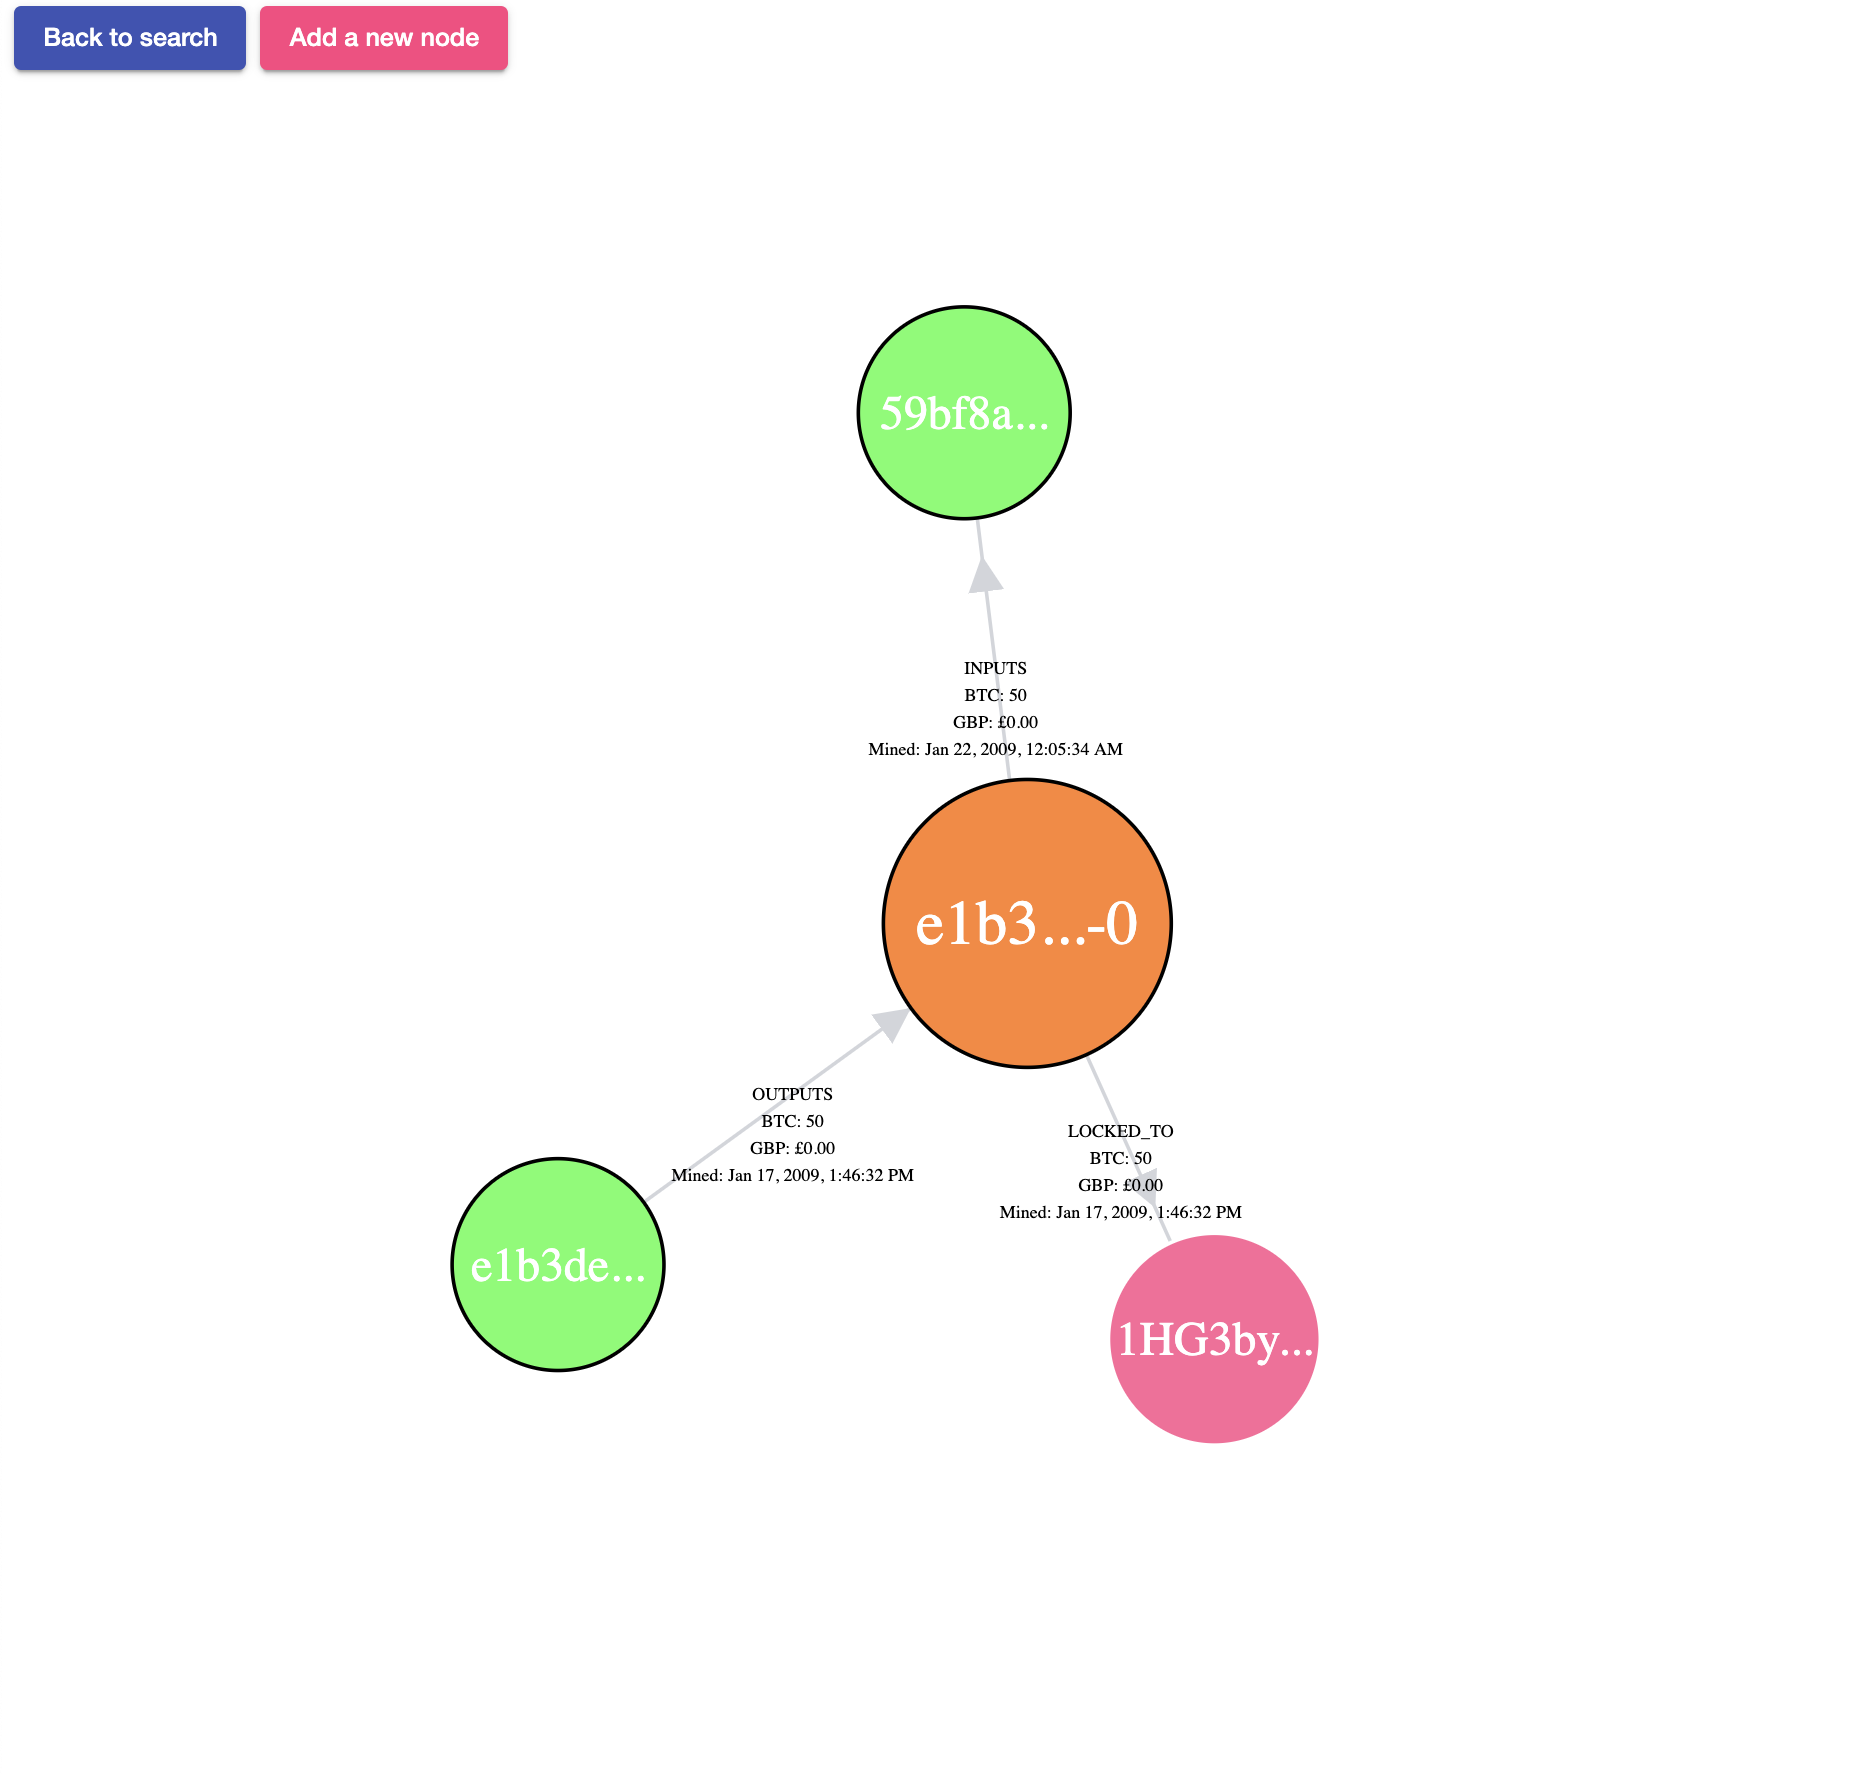
\includegraphics[width = 15cm]{./figures/ui-screenshots/graph-basic}\\[0.5cm] 
  \caption{A screenshot of the search result produced by the search shown in figure \ref{fig:neo4j-screenshot-search-form}}
  \label{fig:neo4j-screenshot-basic-address-nodes}
\end{figure}

\subsubsection{Node information on hover}
Information associated with each type of node is shown on hover. For example, hovering over a block will provide the time it was mined, its hash and the historical exchange rates at the time of mining (see fig \ref{fig:block-info-on-hover}). The node being hovered over will expand in size to indicate which node the information is being displayed for. There is also an option to dismiss the information box using the cross symbol in the top right corner. 
\\\\
Additionally, clicking on each field in the node information box automatically copys that data to the users clipboard. This further improves the user experience as there exists less steps to copying data (such as long ID's or hashes) for further investigation. The data copied will also be copied without the extraneous surrounding data such as labels, currency symbols or data formatting (specifically, selecting dates will copy the epoch time in milliseconds to the clipboard). 

\begin{figure}[h!]
  \centering
  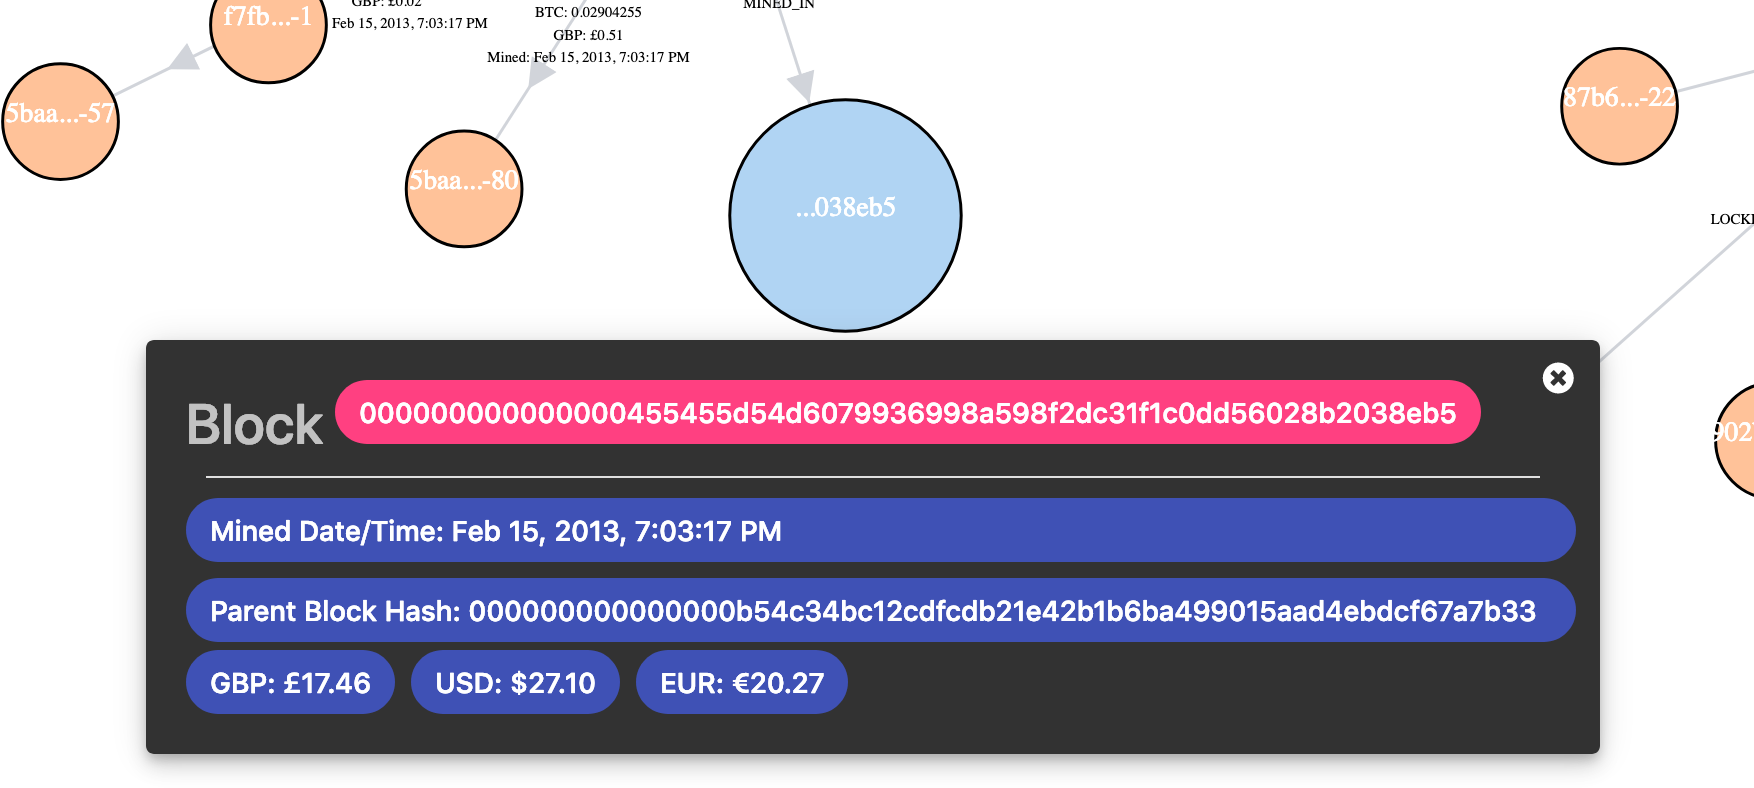
\includegraphics[width = 15cm]{./figures/ui-screenshots/block-info}\\[0.5cm] 
  \caption{A screenshot of block information being displayed when hovering over a block node}
  \label{fig:block-info-on-hover}
\end{figure}

\subsubsection{Link Data}
A primary use of the investigation tool will be to investigate the flow of funds; it is therefore important to make this information visible and digestible. Therefore, each link representing a flow of funds (between \texttt{OUTPUT} and \texttt{TRANSACTION} nodes) displays the value of the funds in BTC and whichever fiat currency the user selects as their preference when searching (GBP, EUR, USD). The link data also provides a timestamp representing the time the transaction was included in the blockchain; this provides context to the value of the output respective to their fiat currencies. 
\\\\
The screenshot shown in figure \ref{fig:link-data} exemplifies the importance of a fiat currency conversion: the same unit of 0.5 BTC is output by transaction \texttt{432f18...} as is input into transaction \texttt{96455e...}, however their equivalent fiat value in USD is dramatically different at $\$1,688$ when the output is produced and $\$2,102$ when the output is spent. The timestamp will also provide context around the timeline of this transfer of funds, in addition to possibly explaining differences in fiat currencie exchange rates.

\begin{figure}[h!]
  \centering
  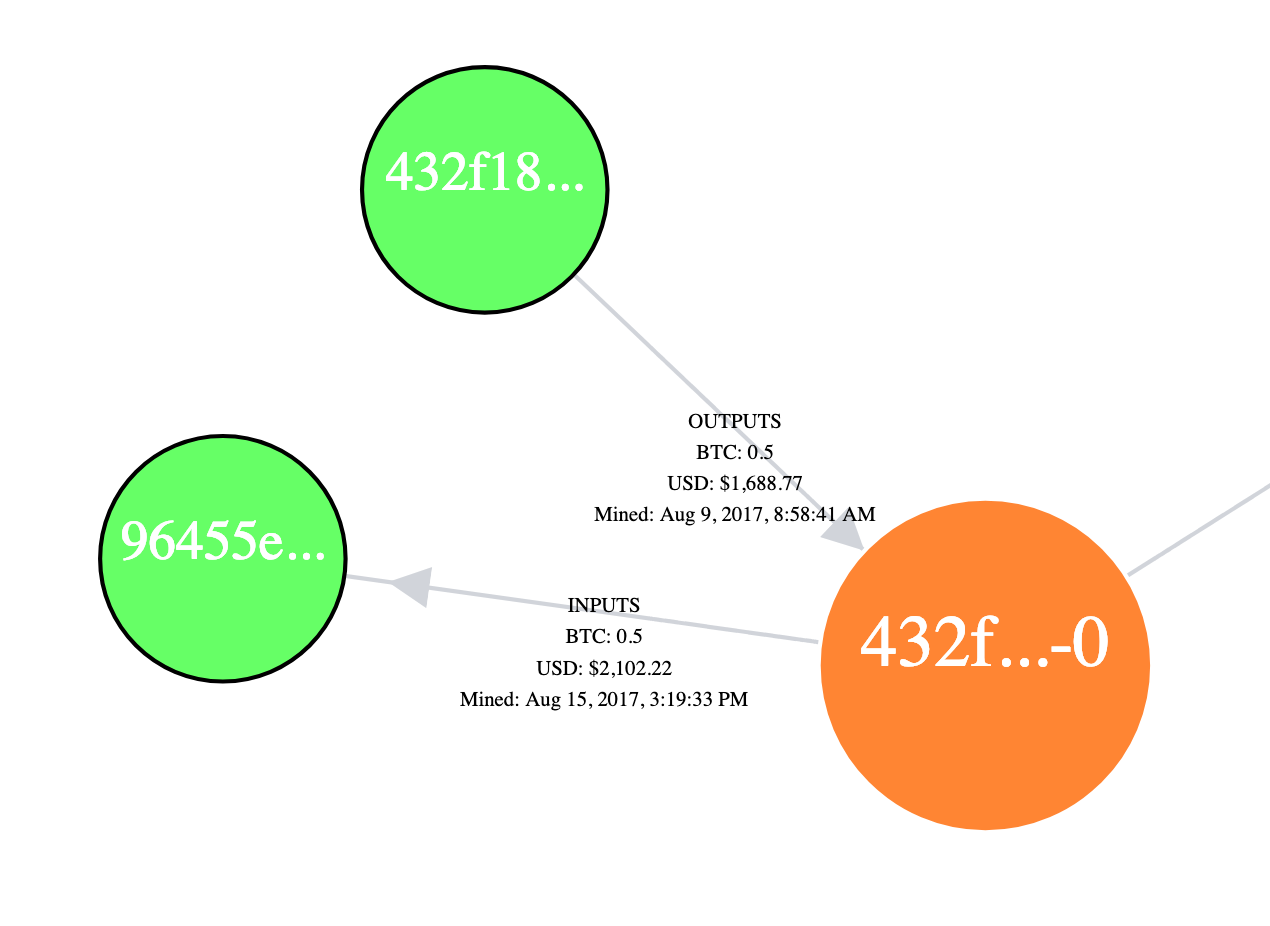
\includegraphics[width = 15cm]{./figures/ui-screenshots/link-data}\\[0.5cm] 
  \caption{A screenshot link data between two transaction nodes (green) and an output node. 
  Transactions IDs are: \texttt{432f18aa46626934c45805046f9c9791fb60bd41da1eb951b47f73bb3b8c7484},\\\texttt{96455e8b6a877f273d14aa13ecb1971577c0d17716b7028c9809c7ca3e1f6e3c}}
  \label{fig:link-data}
\end{figure}

\subsubsection{Traverse the Graph}
Double clicking on a node initiates a request to load that nodes immediate neighbours. Once the request receives a response, the nodes neighbours are added to the existing graph as new nodes and the necessary links are created. Each new node can then also be double clicked and the process will recurse. 
\\\\
Sometimes the time between initiating a request and receiving a response isn't near instantaneous, perhaps due to demand on the database or a greater response size. Therefore, to feedback to the user that a request has been initiated, to prevent them trying to issue multiple requests or thinking that a node has no neighbours, a node will pulse in size while a request is pending. 
\\\\
Additionally, in an investigation view with many nodes, it may not be clear which nodes already have had their neighbouring nodes requested (those without neighbours, for instance). Therefore, nodes will have a thick black border until their nodes have been expanded (see both green transaction nodes in fig \ref{fig:link-data} and will have their border removed once expanded (see the orange output node in fig \ref{fig:link-data}).

\subsubsection{Link Dependant Colour and Size of nodes}
To indicate the differences in a nodes connectivity among the many other nodes in the graph, a nodes colour and size adjusts based on the number of links it has outgoing and incident on it. The rate at which a nodes colour and size changes is normalised by the total number of links in the graph. A node with 30\% of the links in a graph of 10 links should have the same size/colour as a node with 30\% of the links in a graph with 100 links. This feature helps with visualising potentially more important nodes in a graph, and also assists with visual arrangement, by creating a greater circumference to place neighbouring nodes around a node with many links. 
\\\\
An example of this can be seen in figure \ref{fig:address-nodes-colour-size-change} where an address \texttt{1HJtS7...} has more links than another address \texttt{1HeYaB...} and therefore has a higher colour density and larger radius. The figure also exemplifies this for output node \texttt{b777...0} which has more links than the other output nodes, and is therefore slightly larger and of a higher density colour.

\begin{figure}[h!]
  \centering
  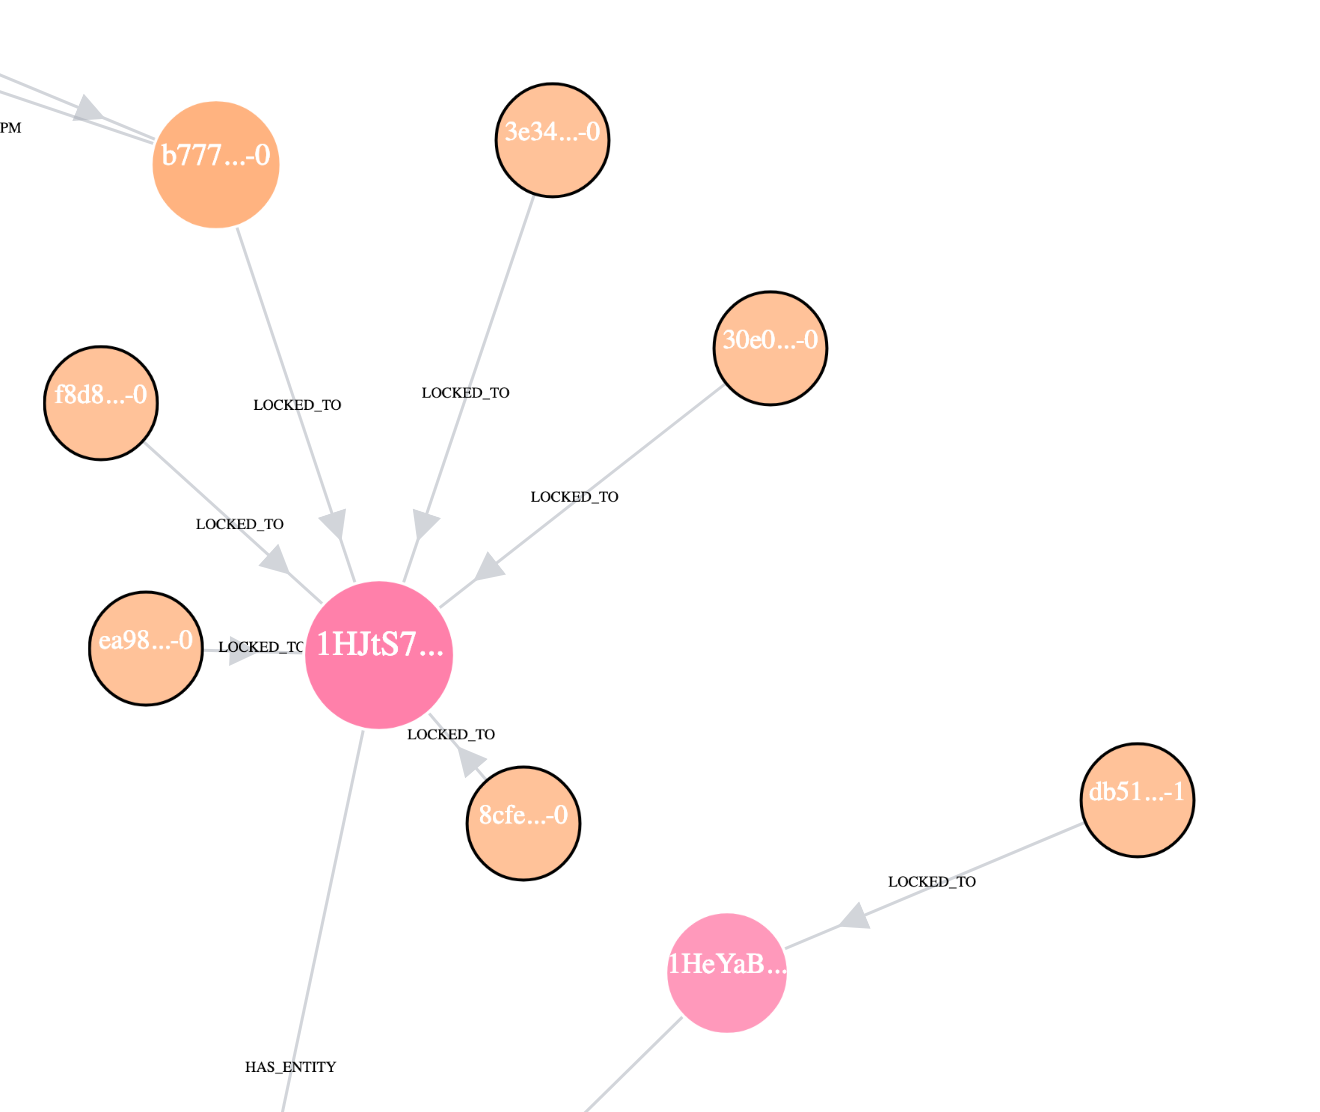
\includegraphics[width = 10cm]{./figures/ui-screenshots/link-dependant-size-colour}\\[0.5cm] 
  \caption{A screenshot of two address nodes, with a varying number of links each.
  Address IDs are: \texttt{1HJtS7wLaqdZRf1Cd4FfJDEWL17VJVDcm2},\\\texttt{1HeYaB7gntUXQBtLaeJmqWzAdFf2PWMEfZ}}
  \label{fig:address-nodes-colour-size-change}
\end{figure}

\subsubsection{Selecting Fiat Currencies}
The Link Data feature, as shown in figure \ref{fig:link-data} displays the fiat currency conversion of output values. The fiat currency is configurable from the address search form, as shown in figure \ref{fig:select-fiat-currencies}. See figure \ref{fig:select-fiat-currencies-gbp} and \ref{fig:select-fiat-currencies-usd} for the graph differences when selecting USD or GBP. 

\begin{figure}[h!]
  \centering
  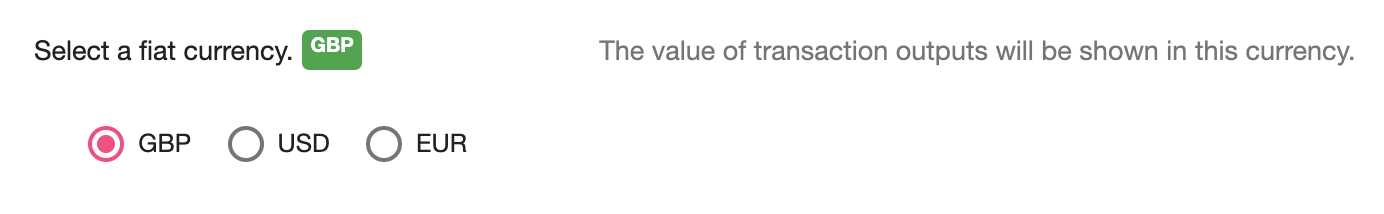
\includegraphics[width = 15cm]{./figures/ui-screenshots/fiat-currency-selection}\\[0.5cm] 
  \caption{A screenshot of a radio button input field of the address search form, allowing one of three currencies to be selected}
  \label{fig:select-fiat-currencies}
\end{figure}
\begin{figure}[h!]
  \centering
  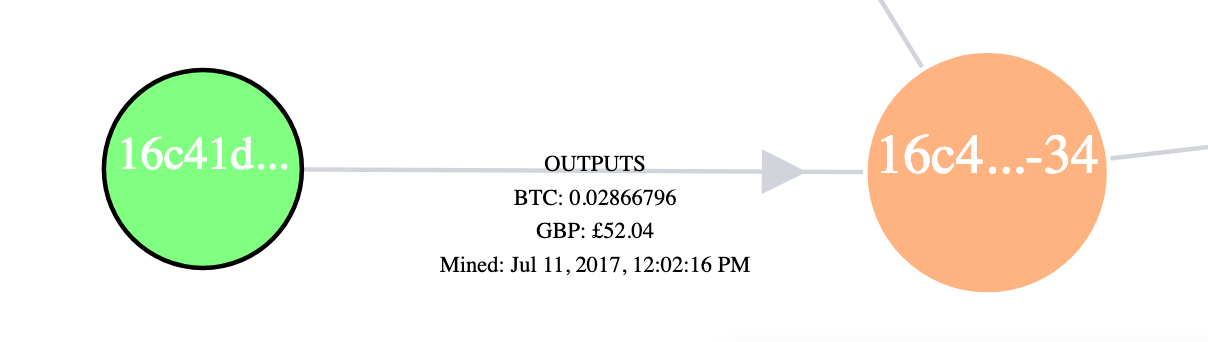
\includegraphics[width = 15cm]{./figures/ui-screenshots/fiat-currency-link-gbp}\\[0.5cm] 
  \caption{A screenshot of link data information displayed in GBP}
  \label{fig:select-fiat-currencies-gbp}
\end{figure}
\begin{figure}[h!]
  \centering
  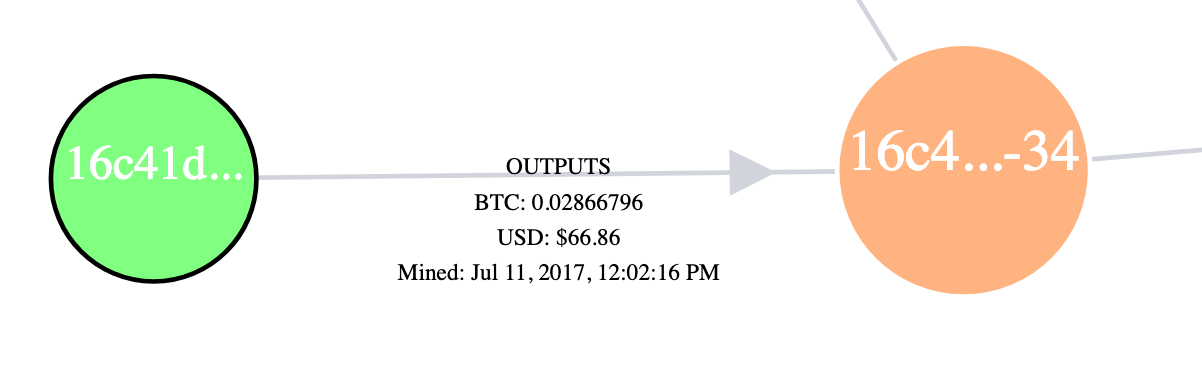
\includegraphics[width = 15cm]{./figures/ui-screenshots/fiat-currency-link-usd}\\[0.5cm] 
  \caption{A screenshot of link data information displayed in USD}
  \label{fig:select-fiat-currencies-usd}
\end{figure}

\subsubsection{Filter Date/Time}
The date/time filter allows the user to specify that they only wish to see transactions/outputs that were mined in the time range specified. The option is disabled by default, but by selecting the toggle button, shown in figure \ref{fig:date-time-filter}, the user can adjust the start and end date/time for the filter. The filtering will remain for any further interactions the user makes when navigating the graph. 

\begin{figure}[h!]
  \centering
  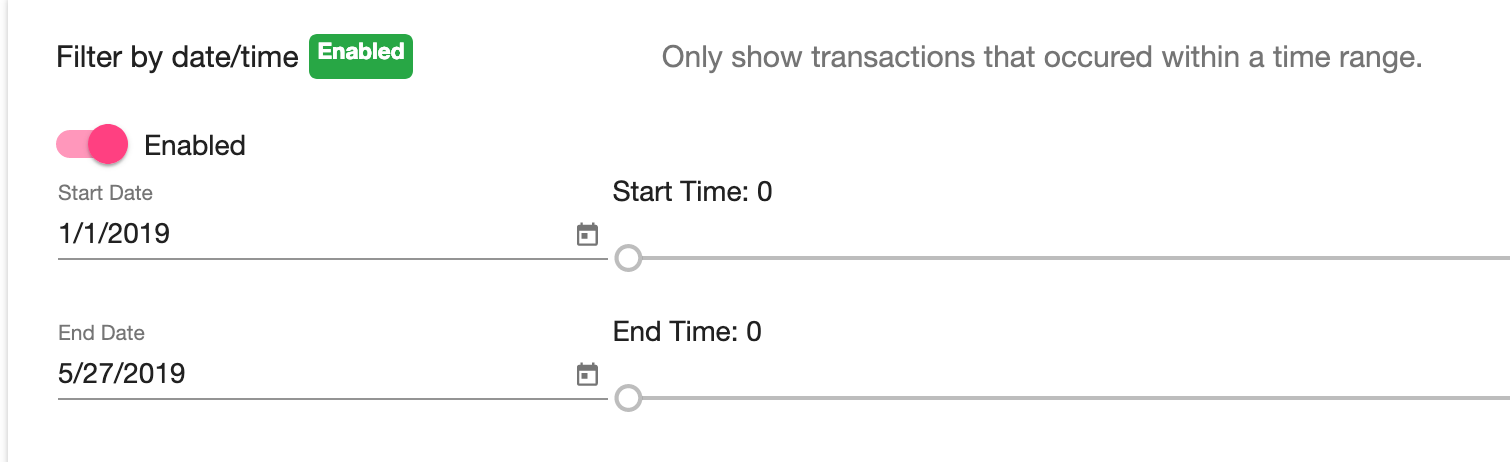
\includegraphics[width = 15cm]{./figures/ui-screenshots/date-time-filter}\\[0.5cm] 
  \caption{A screenshot of the date/time filter input enabled on the search form.}
  \label{fig:date-time-filter}
\end{figure}

\subsubsection{Filter by value, several currencies}
Similar to date filtering, transactions and outputs in the search results can also be filtered by their value. Their value can be filtered either in bitcoin (BTC) or any of the supported fiat currencies (GBP, USD, EUR). Once enabled, only transactions/outputs that have a value that lies in the filter range will be displayed. 

\begin{figure}[h!]
  \centering
  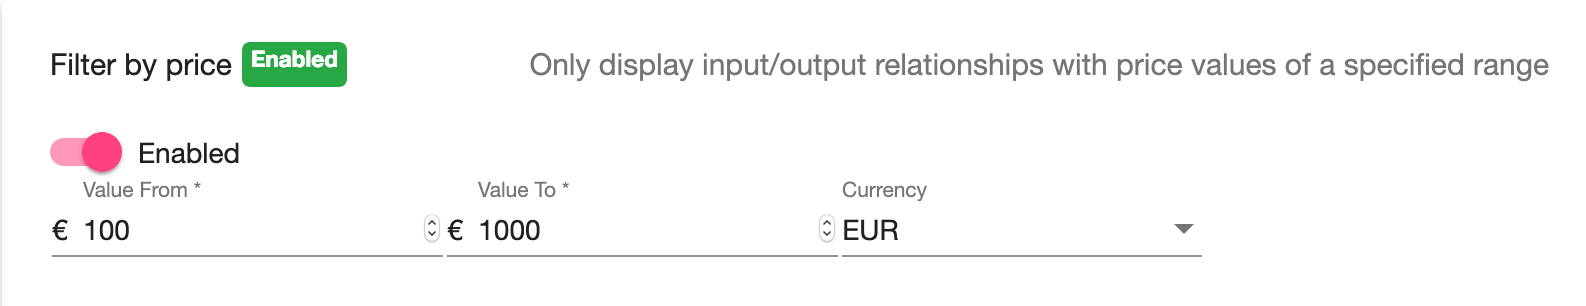
\includegraphics[width = 15cm]{./figures/ui-screenshots/price-filter-form}\\[0.5cm] 
  \caption{A screenshot of the price filter input field.}
  \label{fig:date-time-filter}
\end{figure}

\subsubsection{Limiting nodes}\label{feature-limit-nodes}
Some nodes that are rendered on the graph may have a huge number of neighbours; such as a transaction with many inputs or an entity that has many addresses. If the UI were to attempt to render thousands of nodes using D3, the performance would seriously deteriorate and the web application may become unresponsive. Therefore, in order to prevent this from happening as the default behaviour, the number of nodes that will actually be rendered will be limited, configurable using a field on the search form as shown in figure \ref{fig:limit-node-filter}. The user can disable node limiting completely, and is shown a warning when they do so (see  figure \ref{fig:limit-node-filter-warning}. They can also drag a slider to easily configure the number of nodes to render. 

\begin{figure}[h!]
  \centering
  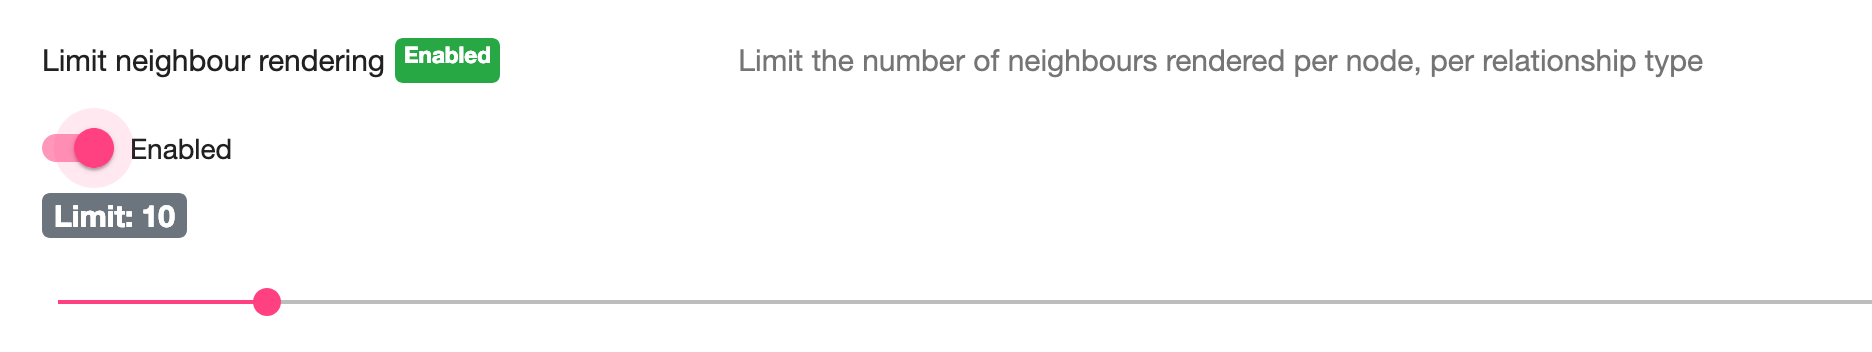
\includegraphics[width = 15cm]{./figures/ui-screenshots/limit-nodes-filter}\\[0.5cm] 
  \caption{A screenshot of the node limiting input field.}
  \label{fig:limit-node-filter}
\end{figure}

\begin{figure}[h!]
  \centering
  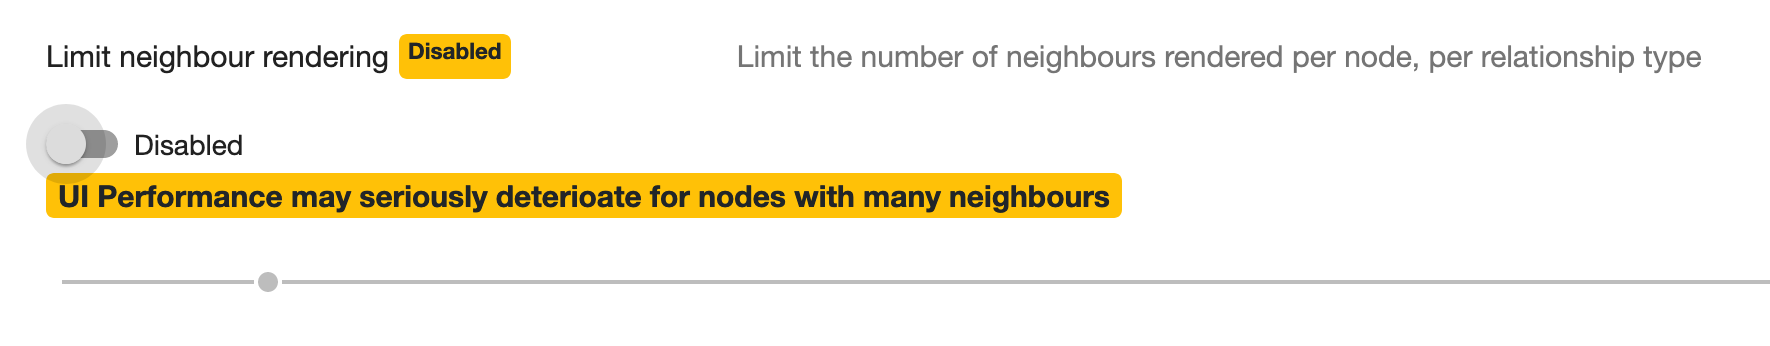
\includegraphics[width = 15cm]{./figures/ui-screenshots/limit-nodes-filter-warning}\\[0.5cm] 
  \caption{A screenshot of the node limiting input field when disabled and showing a warning.}
  \label{fig:limit-node-filter-warning}
\end{figure}

\subsubsection{Enable Multi-input clustering view}
The final option available on the search form is one labelled 'Input Clustering' which is a simple toggle, disabled by default, that the user can turn on when performing a search. Enabling this option will now display 'supernodes' rather than address nodes whenever addresses can be clustered; either through using the same-input heuristic as described in section \ref{section-clustering} or using entity tagging data as described in section \ref{section-entity-tagging}.
\\\\
For example, an address that belongs to the wallet 'BitKonan.com' is \\\texttt{1GEp9Fui9XmyVhszPzFazdW3WHyt1adLR6}. When searching for this address, with the clustering option enabled, the search result will be shown with a large supernode for the wallet, rather than the individual address, as shown in figure \ref{fig:entity-tagging-supernode}. The output nodes connected to the supernode will be all of the outputs for each of the addresses belonging to the supernode. The addresses belonging to the supernode can be viewed by hovering over the node, where the node data component will display them as a list, as shown in figure \ref{fig:entity-tagging-supernode-address-list}.
\\\\
For an address that does not belong to a known entity, but can be linked with other addresses using the multi-input clustering heuristic from section \ref{section-clustering}, then a similar super node will appear, with all of the outputs associated with each address in the cluster rendered as neighbours. 
\\\\
Similar to limiting the number of outputs and transactions to render, the number of clustered addresses and linked outputs displayed is also limited when rendering supernodes. This prevents clustering 'on-demand' as described in section \ref{section-clustering} from taking an unreasonable amount of time, while also providing the option to the user to disable the limiting from the search form and obtaining a complete response. 

\begin{figure}[h!]
  \centering
  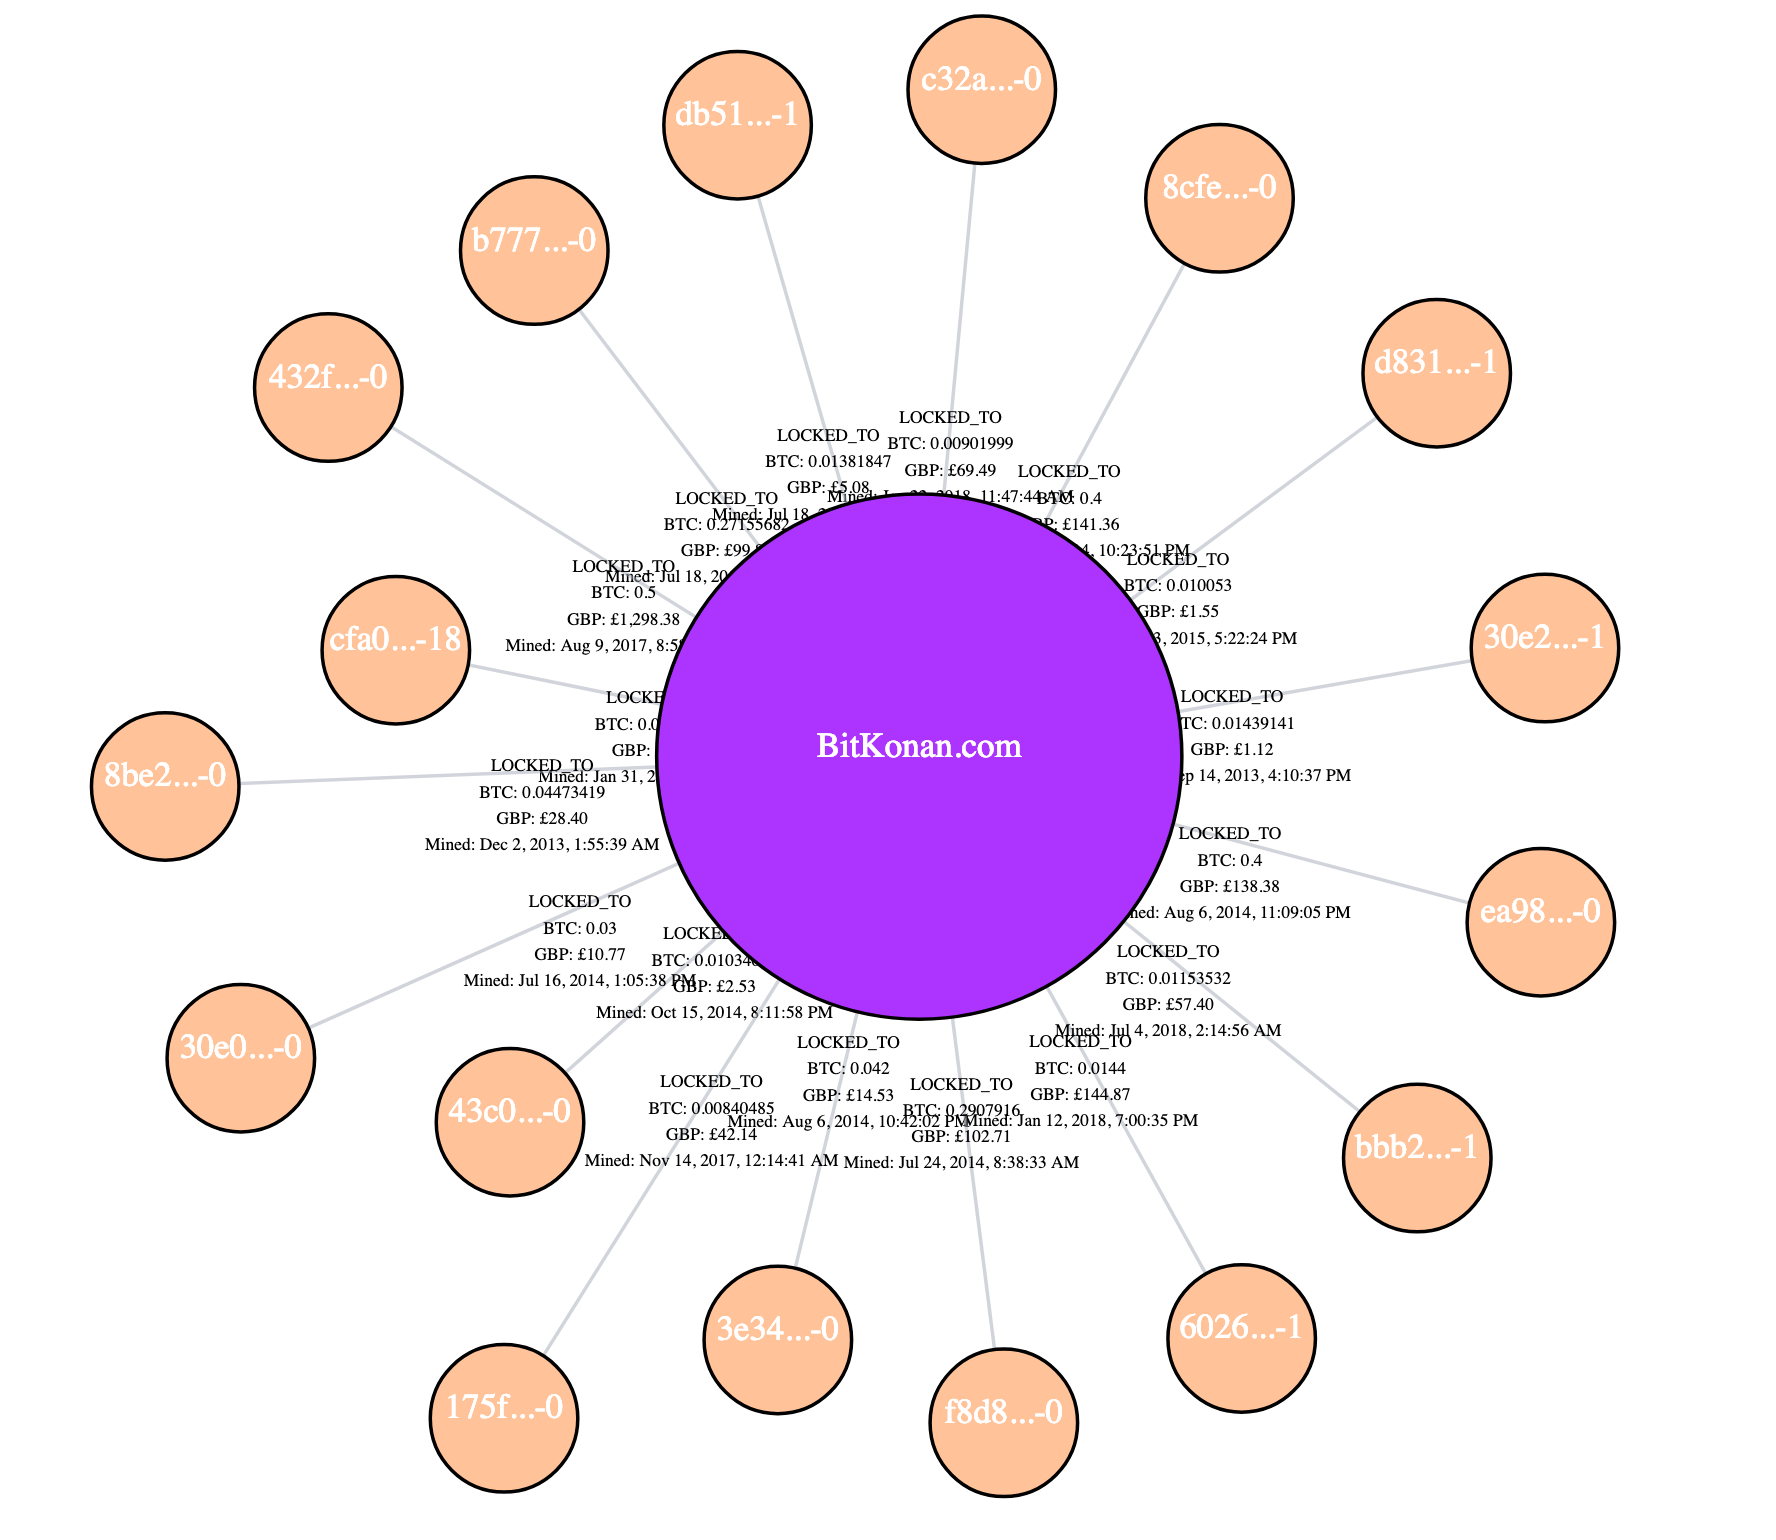
\includegraphics[width = 15cm]{./figures/ui-screenshots/entity-tagging-supernode}\\[0.5cm] 
  \caption{A screenshot of a supernode being displayed for address \texttt{1GEp9Fui9XmyVhszPzFazdW3WHyt1adLR6}.}
  \label{fig:entity-tagging-supernode}
\end{figure}

\begin{figure}[h!]
  \centering
  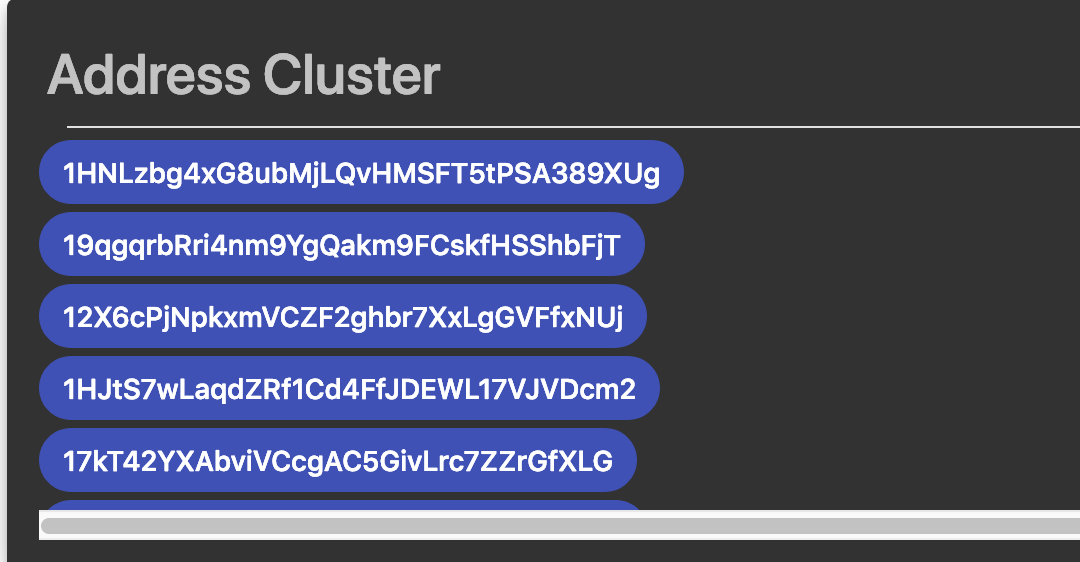
\includegraphics[width = 10cm]{./figures/ui-screenshots/supernode-address-list}\\[0.5cm] 
  \caption{A screenshot of the node data component showing a list of addresses included in a supernode.}
  \label{fig:entity-tagging-supernode-address-list}
\end{figure}

\subsubsection{User Input Validation \& Feedback}
User input validation exists across all forms in the web-app. This includes forms for searching by address, path finding, adding a new node and creating a link. Examples of input validation in the application includes highlighting fields in red and displaying a useful message, such as:
\begin{itemize}
    \item Path Finder Form : No paths found between addresses (if a path does not exist)
    \item Address Search Form : 404, Entity not found (if address does not exist)
\end{itemize}

Additionally, to convey loading states, search forms display a animated loading bar while waiting for a request to return from the backend API. This becomes particularly important for requests that have many linked addresses through clustering and responses can take a number of seconds. For requests made by double clicking a node, a pulsing animation of the node signals that a request is pending.

\subsubsection{Add custom nodes}
It is possible to add custom nodes to the graph. The intention of this feature is the nodes will contain information to complement an active investigation; usually this data will have an off-chain source. There exists various custom node types, based on the typical types of off-chain data that may exist in an investigation. One of these types is photographic ID, which provides the option to upload an image to be displayed in a custom node. The form for adding a new custom node of photographic id type can be seen in figure \ref{fig:add-passport-form}. The user can additionally choose to define an arbitrary number of custom fields in a key, value format. 


\begin{figure}[h!]
  \centering
  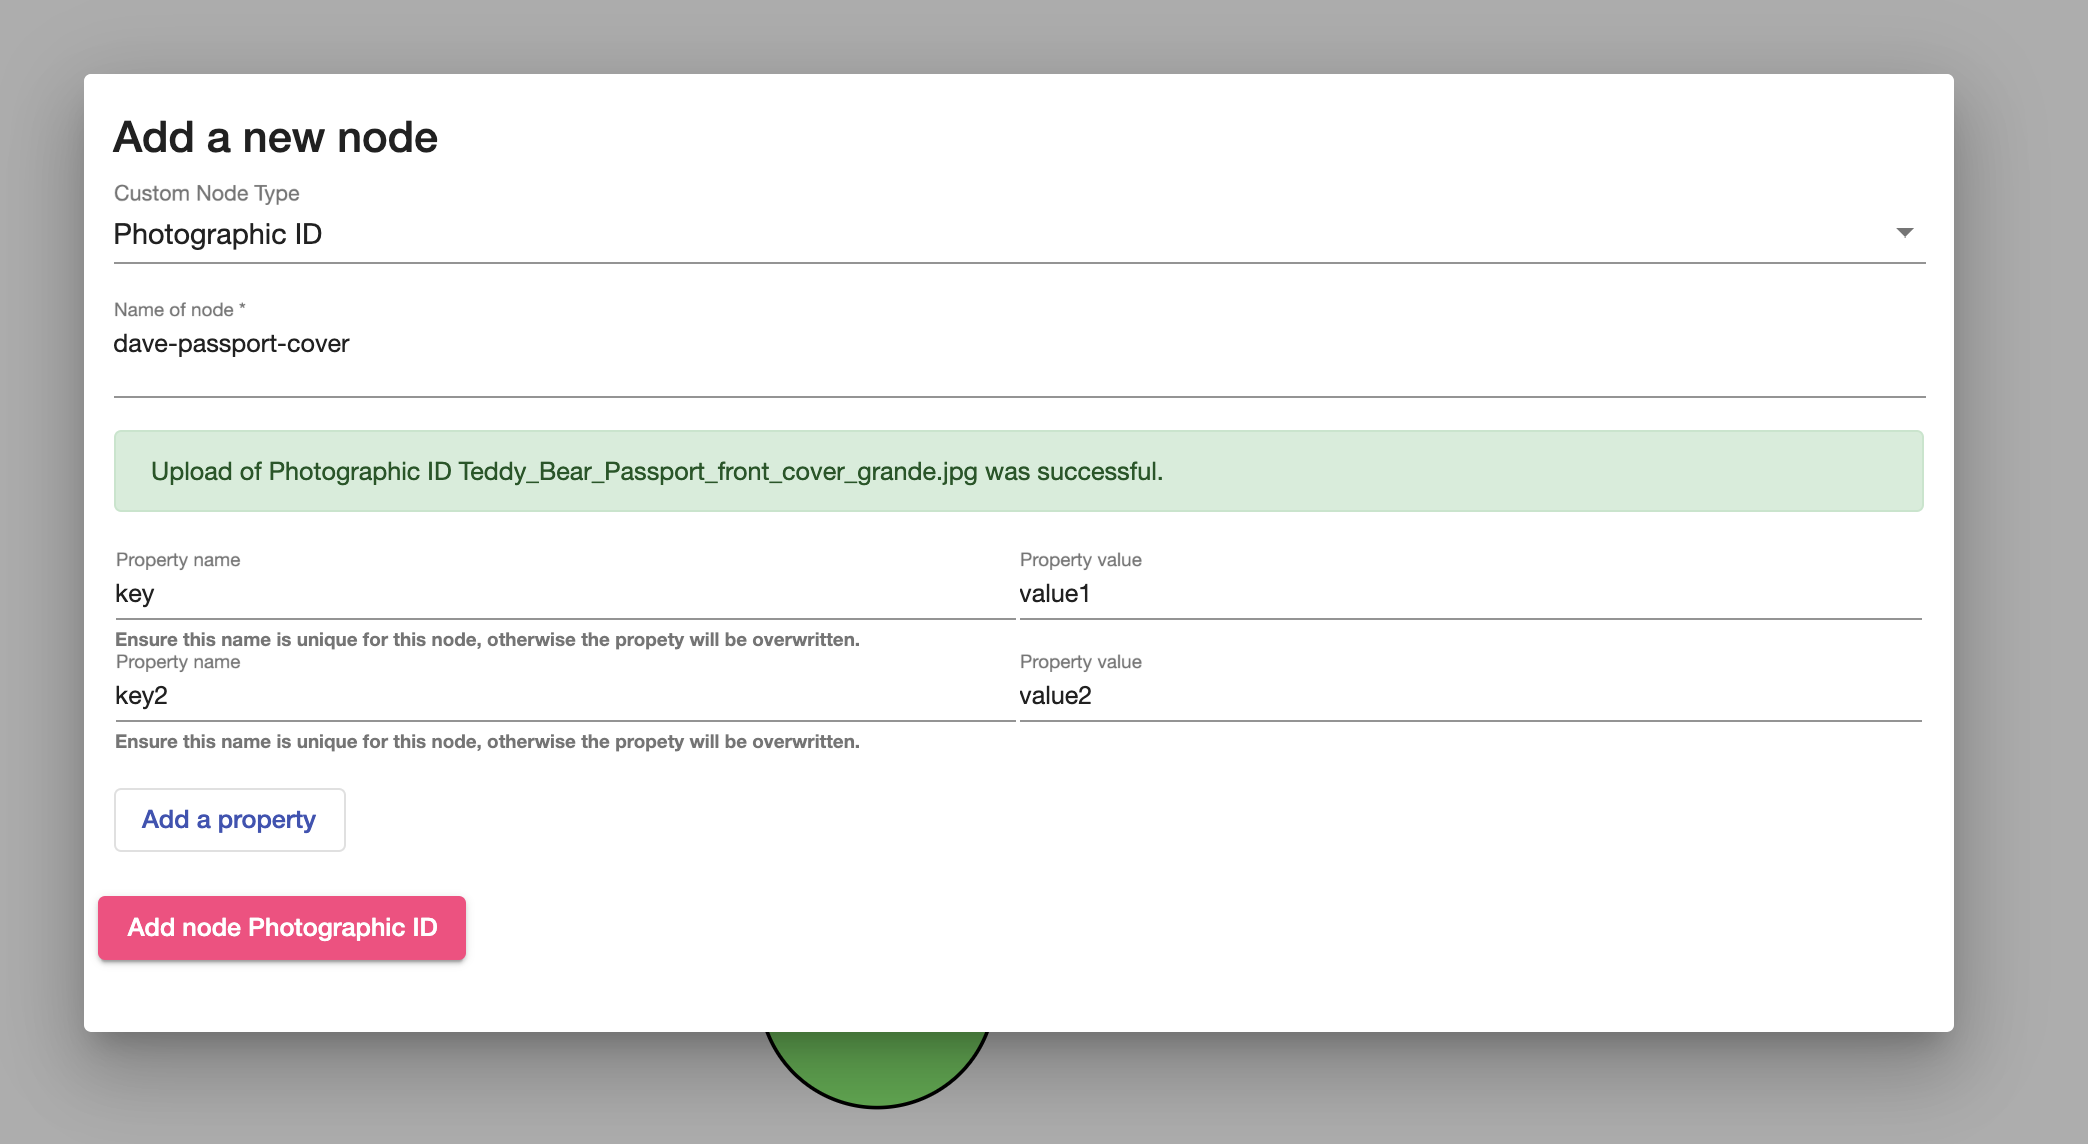
\includegraphics[width = 10cm]{./figures/ui-screenshots/add-passport-form-success}\\[0.5cm] 
  \caption{A screenshot of the form to add a custom node for passport data.}
  \label{fig:add-passport-form}
\end{figure}


\subsubsection{Link custom nodes to other nodes}
Once a custom node exists, it can be associated with any other node shown on the graph. The user can achieve this by hovering over the custom node, so that the node data view displays, as shown in figure \ref{fig:custom-node-data}. This will open a view to introduce the new link, where the user can type the ID of the node they wish to create a link with. To help simplify this process, the target node will have a filtered autocomplete for all of the ID's that currently exist on the graph. The user can also change the direction of the link using the middle arrow button. The link name can then be any custom string defined by the user, and will show on the link as shown in figure \ref{fig:custom-link-graph}

\begin{figure}[h!]
  \centering
  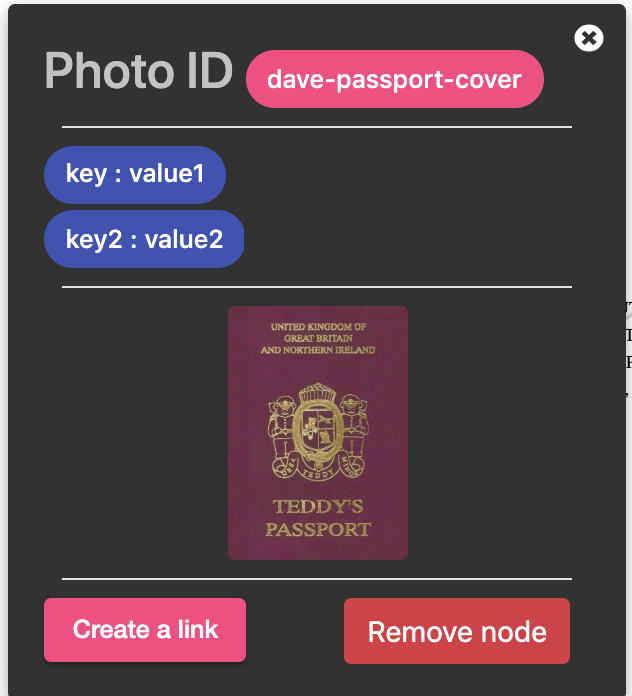
\includegraphics[width = 10cm]{./figures/ui-screenshots/custom-node-data}\\[0.5cm] 
  \caption{A screenshot of the custom node data component.}
  \label{fig:custom-node-data}
\end{figure}


\begin{figure}[h!]
  \centering
  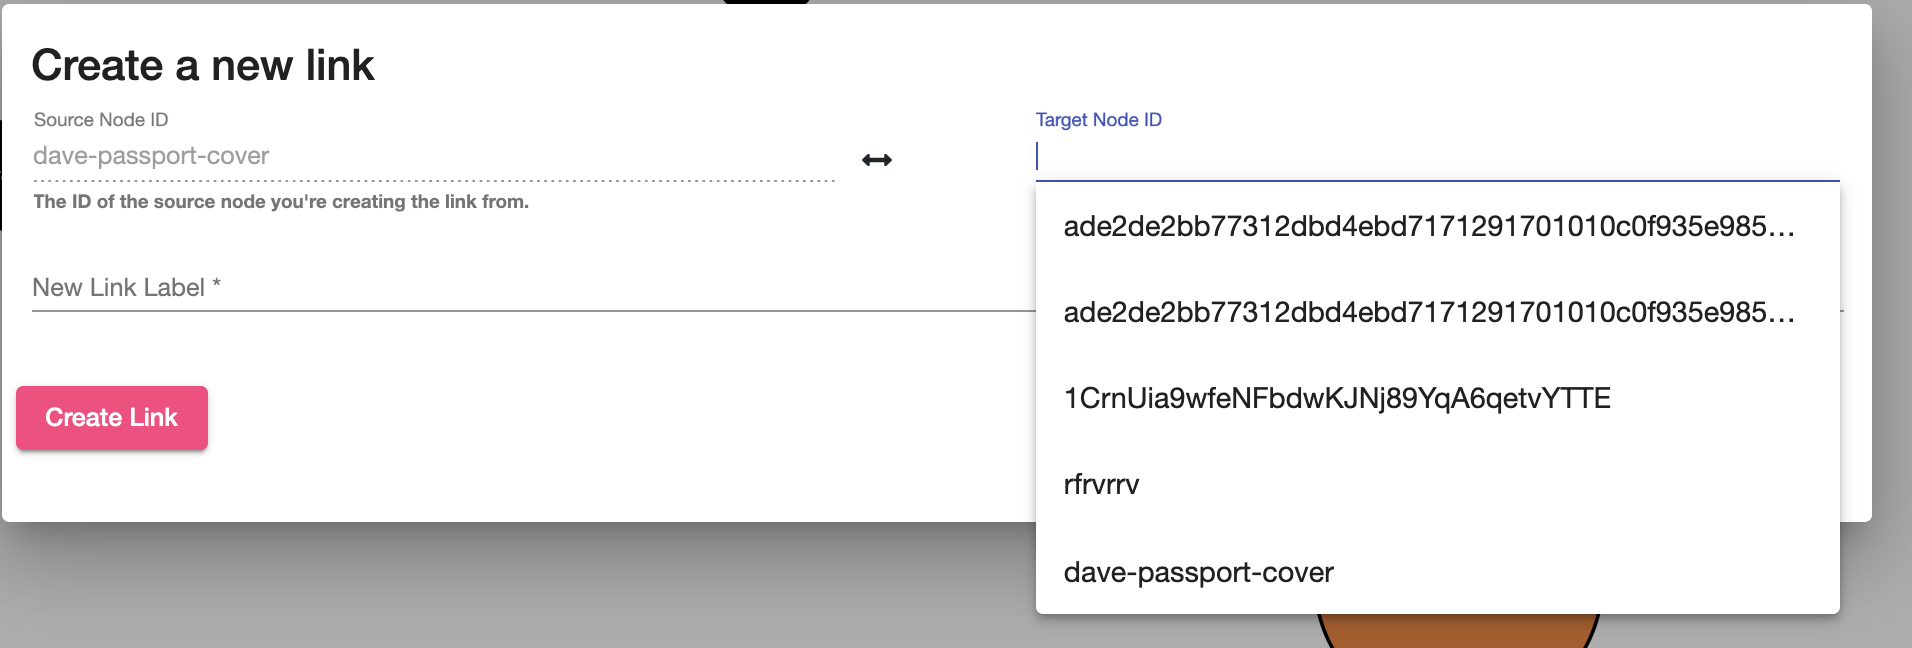
\includegraphics[width = 15cm]{./figures/ui-screenshots/add-link-form}\\[0.5cm] 
  \caption{A screenshot of the form to add a new link from a custom node.}
  \label{fig:add-link-form}
\end{figure}

\begin{figure}[h!]
  \centering
  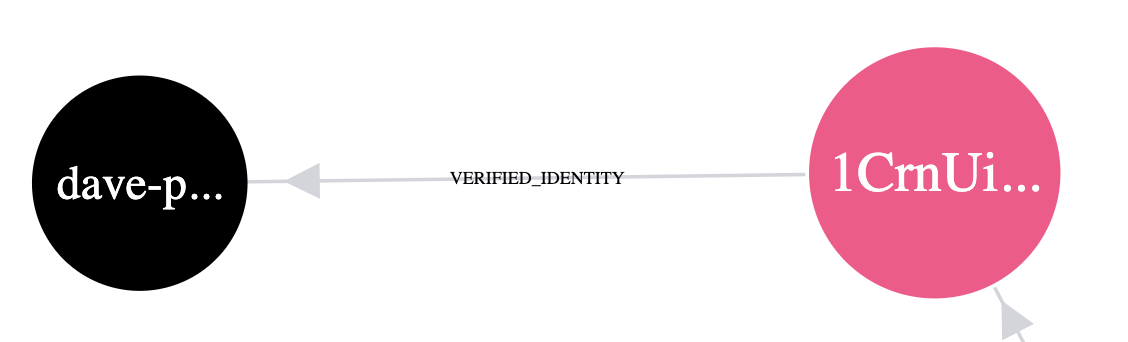
\includegraphics[width = 15cm]{./figures/ui-screenshots/custom-link-graph}\\[0.5cm] 
  \caption{A screenshot of the graph after a new link \texttt{VERIFIED\_IDENTITY} has been introduced between the custom node and an address node.}
  \label{fig:custom-link-graph}
\end{figure}

\subsubsection{Path Finding}
The path finder feature allows the user to search for all paths between any two valid addresses. The path can include paths that contain relationship types \texttt{INPUTS}, \texttt{OUTPUTS} or \texttt{LOCKED\_TO}. This helps identify how two addresses may be linked through the transfer of funds. The result is shown on the graph by only rendering the two address nodes and the intermediate nodes on the path, with the path highlighted in red. A user can expand out neighbouring nodes as usual by double clicking on nodes. An example search result can be seen in figure \ref{fig:path-search-result}. The two addresses shown are clearly connected by the funds they input into the same transaction. 

\todo{better example}
\begin{figure}[h!]
  \centering
  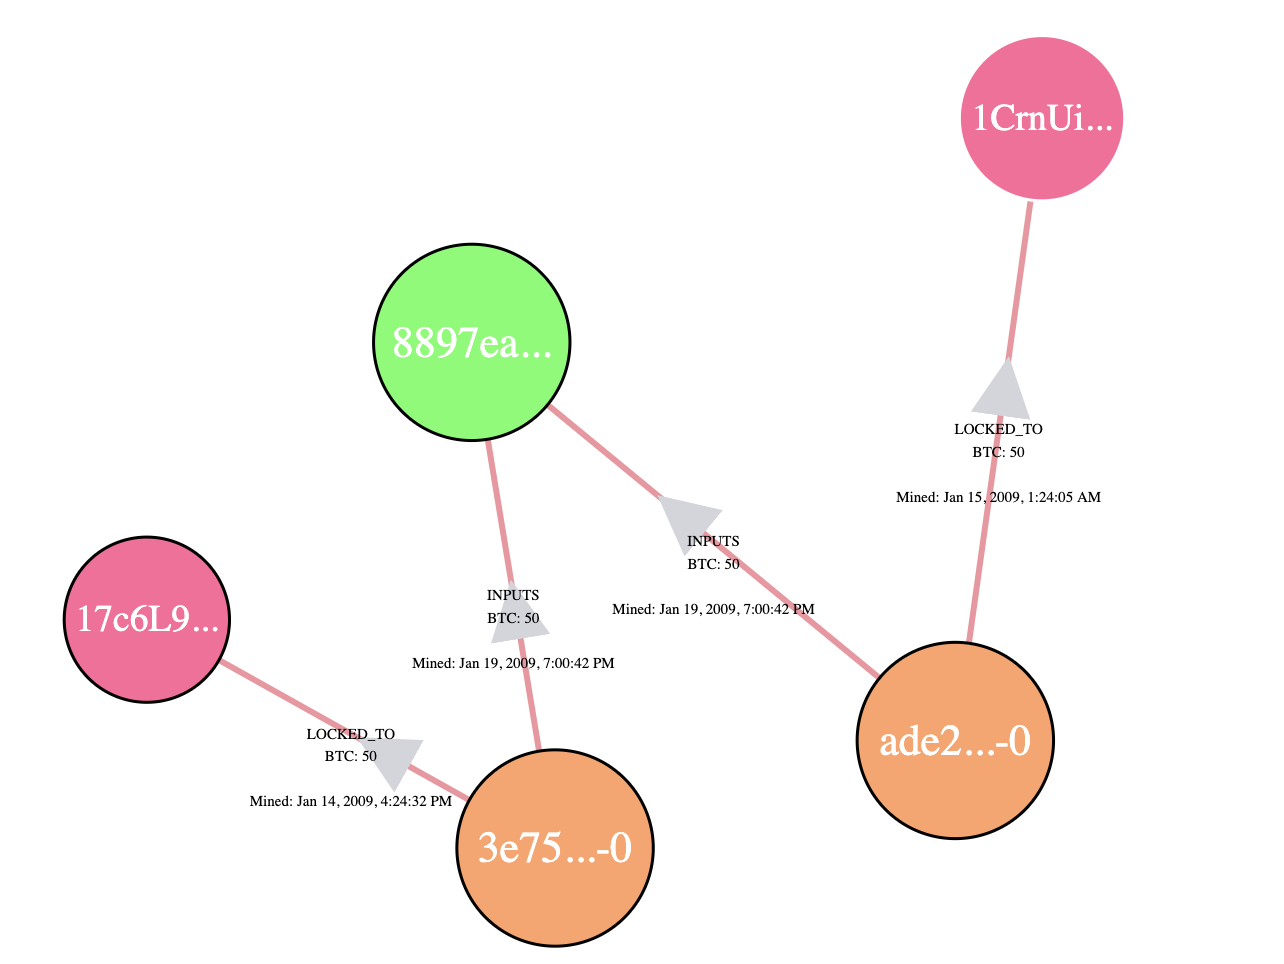
\includegraphics[width = 15cm]{./figures/ui-screenshots/path-find-result}\\[0.5cm] 
  \caption{A screenshot of the result of a path finder search between addresses \texttt{17c6L9JUGVenn6CfqXuB93L3Tk8Tbzefui} and \texttt{1CrnUia9wfeNFbdwKJNj89YqA6qetvYTTE}.}
  \label{fig:path-search-result}
\end{figure}



\subsubsection{Persisting Data}
Instances where data needs to be persisted, such as when a user is uploading an image when creating a custom identification node, are handled by a simple web server implemented using expressjs. 
\\\\
I built a simple API to serve the purpose of uploading images.
\begin{lstlisting}
POST /api/upload/{file}
\end{lstlisting}
This simply stores the file with its file name where the web server is located; allowing the files uploaded to be served as assets in the UI. 